\documentclass[a4paper,10pt]{article}

\usepackage{ucs}
\usepackage[utf8]{inputenc}
%\usepackage{babel}
%\usepackage{graphicx}
\usepackage{fontenc}
\usepackage[pdftex]{graphicx}

\usepackage[pdftex]{hyperref}

\author{Cow Mc.Cow}
\title{Cows}
\date{09/14/17}


\begin{document}
 
 
\maketitle
  
 \begin{center}
  \texttt{edvinjakobsson5@gmail.com}
 \end{center}


 
\section{Section}

Cow cow cow cow Cow.

\subsection{subsection}
 
 \begin{figure}[h]
\begin{center}
 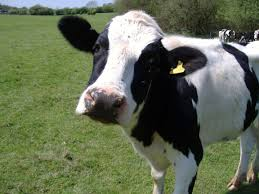
\includegraphics{cow.jpeg}
 \caption{several cows}
\label{cowpicture}
 \end{center}
\end{figure}

Cow cow cow cow cowcow cow.

\section{cowcow}

cow cow \footnote{cow cow cowcow}

\begin{table}[ht]
 \begin{center}
  \caption{cow table}
  \label{tablecow}
  \begin{tabular}{l|c|c|r}
\textbf{left cow}&&&\textbf{right cow}\\
cow &cow&cows&cow \\
 \end{tabular}

 \end{center}

\end{table}

\section{cow math}

\begin{equation}
 cows = \sum\limits_i cow
\end{equation}

\begin{equation}
\label{equation}
cow \left( cowcow  \right) = cow
\end{equation}

cow cow in equation \ref{equation} is cow.

\section{Cows in a row}

\begin{itemize}
 \item cow
 \item cow
 \item cowcow
 \begin{enumerate}
  \item cow 
  \item cowcow cow
 \end{enumerate}
 \item cow

\end{itemize}

\subsection{cows done listed}

cow cow and more:

\begin{verbatim}
cow
\end{verbatim}

\section{reference cows}

\begin{thebibliography}{99}
\bibitem{cowc} cow cow cowcow cow cow cow cccccccc
\end{thebibliography}


 
\end{document}
